\documentclass[xcolor=table]{beamer}
% common packages

\usepackage[utf8]{inputenc}
\usepackage[T1]{fontenc}

\usepackage{aurical}
\usepackage{mathptmx}
\usepackage[scaled]{helvet}
\usepackage{lmodern}
\usepackage{textcomp}
\usepackage[scaled=.88]{DejaVuSansMono}

\usepackage[ngerman]{babel}
\usepackage[german=guillemets]{csquotes}

\usepackage{amsmath}
\usepackage{nicefrac}

\usepackage{tikz}
\usetikzlibrary{positioning,%
  shapes.geometric,%
  shapes.misc,%
  calc,%
  fit,%
  decorations,%
  decorations.pathreplacing,%
  backgrounds,%
  arrows,%
  automata,%
  trees%
}

\usepackage{pifont}
\newcommand{\goodmark}{\textcolor<presentation>{green!50!black}{\Pisymbol{pzd}{52}}}
\newcommand{\badmark}{\textcolor<presentation>{red}{\Pisymbol{pzd}{56}}}

% define colors used by presentation theme AND article
\xdefinecolor{bordeaux}{RGB}{128,0,50}
\xdefinecolor{niceblue}{RGB}{13,41,79}
\xdefinecolor{nicegreen}{RGB}{13,79,18}
\xdefinecolor{niceviolet}{RGB}{79,13,74}
\colorlet{maincolor}{orange}
\colorlet{alertedcolor}{red}
\colorlet{examplecolor}{green!50!black}
\usetheme{latex}

% color system
% - color!9 used as light fill color (e.g. for block content)
% - color!18 used as default fill color (e.g. for state)
% - color!30 used as highlight fill color (e.g. for block header)
% - color!50 used as strong highlight fill color (e.g. for header row)

\usepackage{listings}
\lstdefinelanguage[MyLaTeX]{TeX}[LaTeX]{TeX}%
  % TeX commands
  {moretexcs={enquote,includegraphics,%
    part,chapter,section,subsection,paragraph,subparagraph%
    tableofcontents,listoffigures,listoftables,maketitle,%
    subsection,subsubsection,paragraph,autoref,it,%
    textcolor,colorbox,xdefinecolor,colorlet,foreach,%
    rowcolors,rowcolor,lstdefinestyle,lstset,KOMAoptions,%
    setkomavar,setkomavar*,opening,closing,encl,%
    lehead,cehead,rehead,lefoot,cefoot,refoot,%
    lohead,cohead,rohead,lofoot,cofoot,rofoot,%
    ohead,chead,ihead,ofoot,cfoot,ifoot,%
    areaset,color,%
    automark,manualmark,markright,markboth,%
    tableofcontents,url,clearscrheadfoot,pagemark,headmark,%
    setheadtopline,setkomafont,setheadsepline,setfootsepline,%
    setfootbotline,chaptermark,thesection,thechapter,%
    thesubsection,subtitle,inst,section*,subsection*,institute},%
  % LaTeX environments
  morekeywords={[2]lstlisting,document,letter,center,flushleft,%
    flushright,align,itemize,enumerate,description,tabular,
    titlepage,figure,table,frame%
    },%
  % other things (like packages) to highlight
  morekeywords={[3]listings,textcomp,courier,xcolor,scrartcl,%
    scrlttr2,inputenc,babel,%
    fontenc,lmodern,mathptmx,%
    helvet,geometry,scrpage2,scrreprt,scrbook,%
    article,report,book,hyperref,%
    csquotes,amsmath,amssymb,la},
  alsoletter={0123456789*}
  }%

\lstdefinelanguage{BibTeX}
  {keywords={%
      @article,@book,@collectedbook,@conference,@electronic,@ieeetranbstctl,%
      @inbook,@incollectedbook,@incollection,@injournal,@inproceedings,%
      @manual,@mastersthesis,@misc,@patent,@periodical,@phdthesis,@preamble,%
      @proceedings,@standard,@string,@techreport,@unpublished%
      },
   comment=[l][\itshape]{@comment},
   morekeywords={[2]author,title,year,publisher,editor,booktitle,journal,series,volume,number,pages,institution,note,howpublished},
  }

\lstset{%
  basicstyle=\ttfamily,%
  language=[MyLaTeX]TeX,%
  texcsstyle=*\color{violet}\bfseries,%
  keywordstyle=\color{violet}\bfseries,%
  keywordstyle={[2]\color{green!70!black}\bfseries},%
  keywordstyle={[3]\color{maincolor!70!black}\bfseries},%
  commentstyle=\color{gray}\itshape,%
  stringstyle=\itshape,%
  numbers=none,%
  frame=lines,%
  backgroundcolor=\color{maincolor!10},%
  rulecolor=\color{maincolor!70},%
  framerule=1pt,%
  showstringspaces=false,%
  upquote=true,%
  framexleftmargin=3pt,%
  framexrightmargin=3pt}

\lstdefinestyle{pseudo}{language={},%
  basicstyle=\normalfont,%
  morecomment=[l]{//},%
  morekeywords={for,to,while,do,if,then,else},%
  mathescape=true,%
  columns=fullflexible}

\lstdefinestyle{block}{%
  backgroundcolor={},%
  frame=no,%
  aboveskip=0pt,%
  belowskip=0pt
}

% german umlauts and red braces
\lstset{
  literate={ö}{{\"o}}1
           {Ö}{{\"O}}1
           {ä}{{\"a}}1
           {Ä}{{\"A}}1
           {ü}{{\"u}}1
           {Ü}{{\"U}}1
           {ß}{{\ss}}1
           {\{}{{\textbf{\color{red}\{}}}1
           {\}}{{\textbf{\color{red}\}}}}1
           {[}{{\textbf{\color{red}[}}}1
           {]}{{\textbf{\color{red}]}}}1
}

\usepackage{tabularx}

% zebra tables
\newcommand{\mainrowcolors}{\rowcolors{1}{maincolor!30}{maincolor!9}}
\newenvironment{zebratabular}{\mainrowcolors\begin{tabular}}{\end{tabular}}
\newcommand{\setrownumber}[1]{\global\rownum#1\relax}
\newcommand{\headerrow}{\rowcolor{maincolor!50}\setrownumber1}

\AtBeginDocument{\hypersetup{
  pdftitle={\titlestring},
  pdfauthor={\authorstring}}
  \title[\shorttitlestring]{\titlestring}
  \author[\shortauthorstring]{\authorstring}
  \date{\datestring}}

% set texts used later
\newcommand{\targetsname}{Ziele dieses Vortrags}
\newcommand{\targetscontentname}{Ziele und Inhalt}
\newcommand{\outlinename}{Gliederung}

% often used sets
\newcommand{\set}[1]{\mathbb{#1}}
\newcommand{\R}{\set{R}}
\newcommand{\N}{\set{N}}
\newcommand{\Z}{\set{Z}}
\newcommand{\Q}{\set{Q}}

% easier use of operatorname
\newcommand{\op}[1]{\operatorname{#1}}

% display vectors in bold
\let\oldvec\vec
\let\vec\boldsymbol

\newcommand{\xxx}{\only<presentation>{\vskip1em}}

\newcommand{\inhead}[1]{\textbf{\color{maincolor}#1}}

\newenvironment{mybib}{%
  % temporary disable \section command to get rid of bibliography heading
  \renewcommand{\chapter}[2]{}
  \begin{thebibliography}{10}
}{%
  \end{thebibliography}
}

% load logo collection from "Die TeXnische Komödie"
\usepackage{dtklogos}

% load common user macros
\newcommand{\website}{
  \begin{Frame}[t]{Website}
    \alt<presentation>{%
      \vskip-4ex\hfill\parbox{6cm}{\centering
        
\includegraphics[width=6cm]{images/qrcode}\\[1ex]
        \href{http://www.mlte.de/latex}{\huge\texttt{mlte.de/latex}}
      }
      \par\vskip2ex}{%
        Auf der Seite \url{http://www.mlte.de/latex} befinden sich}
    \begin{itemize}
      \item diese Präsentation, das Skript zum Vortrag,
      \item Beispieldokumente, Links zu weiteren Quellen und
      \item der Link zum Github-Repository\only<article>{.}
    \end{itemize}
  \end{Frame}
}

\newcommand*{\icon}[2][2]{%
  \tikz\draw[very thick, line join=round]
    (-.5,.5) -- ++(.7,0) -- ++(.3,-.3) --
    ++(-.3,0) -- ++(0,.3) -- ++(.3,-.3) -- ++(0,-.4)
    \foreach \x in {1,...,#1} {
      -- ++(0,-.2)
    }
    -- ++(-1,0) -- cycle
    (-.5,.2) node[fill, text=white,
      inner sep=2pt, minimum width=8mm, anchor=center] {#2}
    ++ (.1,-.3) -- ++(.8,0) \foreach \x in {1,...,#1} {
      -- ++(0,-.1) -- ++(-.8,0) -- ++(0,-.1) -- ++(.8,0)
    };
}

\colorlet{texicon}{examplecolor}
\colorlet{pdficon}{maincolor}
\colorlet{auxicon}{-examplecolor}
\colorlet{logicon}{black}
\colorlet{bblicon}{-maincolor}
\colorlet{bibicon}{alertedcolor}

\colorlet{tikzexample}{examplecolor!10}

\mode
<article>

\newcommand*{\examplebox}[2][center]{%
  \begingroup%
  \fboxsep=2ex%
  \begin{center}
    \colorbox{tikzexample}{#2}
  \end{center}
  \endgroup}

\mode
<presentation>

\newcommand*{\examplebox}[2][center]{%
  \begingroup%
  \fboxsep=2ex%
  \ifthenelse{\equal{#1}{center}}{%
    \hfill\colorbox{tikzexample}{#2}\hfill%
  }{%
    \colorbox{tikzexample}{#2}
  }%
  \endgroup}

\mode
<all>

\newcommand*{\tikzexample}[2][center]{\examplebox[#1]{%
  \begin{tikzpicture}#2\end{tikzpicture}}}

\newcommand*{\beamerexample}[2][1]{%
  \alt<presentation>{%
    \plain{\includegraphics[page=#1]{#2}}
  }{
    \plain{\frame{\includegraphics[width=10cm,page=#1]{#2}}}
  }
}

\newcommand{\currentauthor}{Malte}
\newcommand{\updateauthorcolors}{\ifthenelse{\equal{\currentauthor}{Malte}}{
  \colorlet{authormalte}{maincolor}\colorlet{authorjonny}{black}
}{
  \colorlet{authormalte}{black}\colorlet{authorjonny}{maincolor}
}}
\newcommand{\insertcurrentauthor}{\currentauthor}
\updateauthorcolors
\newcommand{\malte}{\renewcommand{\currentauthor}{Malte}\updateauthorcolors}
\newcommand{\jonny}{\renewcommand{\currentauthor}{Johannes}\updateauthorcolors}

\newcommand{\lorem}{\textcolor{black!40}{Auch in der zweiten Zeile. Lorem ipsum dolor sit amet, consectetur, adipisci velit, \ldots}}

\newcommand{\colorsample}[1]{\textcolor{#1}{\rule[-.5ex]{2em}{2ex}} \texttt{#1}}








% set options for article
\mode
<article>

\newcommand{\itemref}[1]{#1}
\newcommand{\term}[1]{#1}

\KOMAoption{fontsize}{12pt}
\KOMAoption{parskip}{half}
\KOMAoption{open}{any}
\KOMAoption{headings}{big}
\KOMAoption{numbers}{noendperiod}
\KOMAoption{twoside}{false}
\KOMAoption{mpinclude}{true}

\usepackage{paralist}
% use compactitem as default itemize environment
\newenvironment{looseitemize}{}{}
\let\looseitemize\itemize
\let\endlooseitemize\enditemize
\let\itemize\compactitem
\let\enditemize\endcompactitem
% use compactenum as default enumerate environment
\newenvironment{looseenumerate}{}{}
\let\looseenumerate\enumerate
\let\endlooseenumerate\endenumerate
\let\enumerate\compactenum
\let\endenumerate\endcompactenum

% create head and foot line
\usepackage{scrpage2}
\pagestyle{scrheadings}

% stretch headline above margin (scrguide -- page 244)
\setheadwidth[0pt]{textwithmarginpar}

% create targets block
\usepackage{minitoc}
\nomtcrule
\ktightmtctrue
\tightmtctrue
\setlength{\mtcindent}{0pt}
\mtcsetfont{minitoc}{*}{\normalsize\rmfamily\upshape\mdseries}
\mtcsetfont{minitoc}{section}{\normalsize\rmfamily\upshape\mdseries}
\mtcsetfont{minitoc}{subsection}{\normalsize\rmfamily\upshape\mdseries}
\mtcsettitlefont{minitoc}{\normalsize\sffamily\upshape\bfseries}

\makeatletter
\newcommand{\targets}[1]{
  \parbox[t]{0.46\textwidth}{\raggedright
    \kern-0.8\baselineskip\nopagebreak[4]%
    \par\noindent %%
    \begin{tabular}{@{}p{\columnwidth}@{}}
    \reset@font\mtifont\do@mtitc{\mtc@v\targetsname}\\
    \end{tabular}%
    \begin{mtc@verse}{\mtcoffset}
    \begin{enumerate}#1\end{enumerate}
    \end{mtc@verse}
  }
  \hskip0.04\textwidth
  \parbox[t]{0.48\textwidth}{\raggedright
    \minitoc
  }
  % emulate two frames
  \addtocounter{slidenumber}{2}
  \addtocounter{framenumber}{2}
}
\makeatother

% keep the name of the current chapter and the current section

\clearscrheadfoot % clear all default settings
\automark[chapter]{section} % \automark[\rightmark]{\leftmark}

\ihead{\shorttitlestring\ \rightmark\ \textcolor{maincolor}{\bfseries |} \leftmark \hfill \pagemark}
\setkomafont{pageheadfoot}{\normalfont\sffamily}
\setkomafont{pagenumber}{\usekomafont{pageheadfoot}\color{maincolor}}
\setheadsepline{0.5pt}[\color{maincolor}]


% Create own counter as replacement for framenumber. framenumber is
% incremented in article mode as \refstepcounter{framenumber} by
% beamer and hyperref complains about duplicated targets if framenumber
% gets resetted after each chapter.
\newcounter{slidenumber}

\makeatletter
% create AtBeginChapter analog to AtBeginDocument
\def\AtBeginChapter{\g@addto@macro\@beginchapterhook}

\@onlypreamble\AtBeginChapter

\let\oldchapter\chapter
\long\def\chapter{\@beginchapterhook
  \oldchapter}
  
\ifx\@beginchapterhook\@undefined
  \let\@beginchapterhook\@empty
\fi
\makeatother

% slidenumbers starts over with every new chapter with 2 on chapterframe
\AtBeginChapter{\setcounter{slidenumber}{2}}

% hide block title in article mode
\setbeamertemplate{block begin}{}
\setbeamertemplate{block end}{}

% display block title in Block environment
\newenvironment{Block}{%
  \setbeamertemplate{block begin}[default]
  \setbeamertemplate{block end}[default]
  \begin{block}}{\end{block}}

% hide frame title and subtitle in article mode for default frame environment
\setbeamertemplate{frametitle}{}

% display frame title of Frame environment
\newenvironment{Frame}{%
  \setbeamertemplate{frametitle}{%
    \paragraph*{%
      \insertframetitle%
      \ifx\insertframesubtitle\empty\else%
        \newline%
        \mdseries\insertframesubtitle%
      \fi%
    }\ \par}
  \begin{frame}}{\end{frame}}

% hide effect of beameritemize
\newenvironment{beameritemize}{%
  \let\item\relax\ignorespaces}{%
  \ignorespacesafterend}
  
% map beamerenumerate to inparaenum
\newenvironment{beamerenumerate}{%
  \begin{inparaenum}\ignorespaces}{%
  \end{inparaenum}\ignorespacesafterend}

% map plain command to frame
\newcommand{\plain}[1]{\frame{#1}}

% display frame number
%\setbeamertemplate{frame end}{%
%  \marginpar{\hfill\scriptsize\sffamily\color{maincolor}$\to\,$\insertframenumber}}

% display framenumber as chapter number and slide number
\renewcommand{\insertframenumber}{\thechapter-\theslidenumber}

% incremend slide number
\setbeamertemplate{frame begin}{\stepcounter{slidenumber}}
% display slide number
\setbeamertemplate{frame end}{%
  \marginpar%
    [\scriptsize\sffamily\color{maincolor}\insertframenumber$\,\leftarrow$\hfill]%
    {\hfill\scriptsize\sffamily\color{maincolor}$\rightarrow\,$\insertframenumber}}
      
\newcommand{\script}{\addtomargin{Script}\mode<article>}
      
\usepackage{hyperref}
\hypersetup{breaklinks=true,
            pdfborder={0 0 0},
            pdfhighlight={/N}}

\usepackage{verbatim} % for the comment environment
















% Set options for beamer
\mode
<presentation>

\makeatletter
% Reverts "Heiko's fix for correct generation of section* and
% subsection* bookmarks" in beamerbasecompatibility.sty which
% disables bookmarks in \section* and \subsection*.
% This is done by disabling \Hy@writebookmark in \beamer@section
% and \beamer@subsection if their second argument is empty.
% This is the case for \section* and \subsection* as these
% commands are mapped to \beamer@section[{#1}]{} resp.
% \beamer@subsection[{#1}]{}. By defining \beamer@section and
% \beamer@subsection again to the original and not patched version
% in the macro \beamer@lastminutepatches where the patch is applied
% this behaviour gets disabled. This is mainly reverted because
% bookmarks of parts are not added after \section*{Conclusion} due
% to this patch.
\g@addto@macro\beamer@lastminutepatches{
  \ifx\org@beamer@section\undefined{}%
  \else
    \let\beamer@section\org@beamer@section{}%
  \fi
  \ifx\org@beamer@subsection\undefined{}%
  \else
    \let\beamer@subsection\org@beamer@subsection{}%
  \fi
}
\makeatother

% display framenumber as part number and frame number
\renewcommand{\insertframenumber}{\thepart-\theframenumber}

% reset frame number at the beginning of each chapter
\AtBeginPart{
  \setcounter{framenumber}{0}
}

\AtBeginSection[]{
  \begingroup
  \setbeamercolor{background canvas}{bg=maincolor!9}
  \plain{
    \Huge\color{maincolor}\bfseries
    \vskip11ex
    \begin{center}
      \insertsection
    \end{center}
    \vfill
    \normalsize
    \hfill\insertcurrentauthor\ \strut
  }
\endgroup
}

\newcommand{\chapter}[1]{
  \part{#1}
  \title{\LaTeX\\#1}
  \plain{
  \begin{center}
    \vskip4ex
    \textbf{\fontsize{36pt}{36pt}\selectfont\rmfamily\color{maincolor}\LaTeX}
    \par\vskip2ex
    \large Johannes und Malte auf der MetaNook 2013
  \end{center}

  \vskip2ex\hskip4em
  \begin{minipage}{20em}\Large
    18:00 Uhr\\
    \tikz[remember picture] \node[coordinate] (n1) {};
    \ \textbf{\color{maincolor}Grundlagen}

    \vskip1ex
    19:15 Uhr\\
    \tikz[remember picture] \node[coordinate] (n2) {};
    \ \textbf{\color{maincolor}Fortgeschrittene Verwendung}

    \vskip1ex
    20:45 Uhr\\
    \tikz[remember picture] \node[coordinate] (n3) {};
    \ \textbf{\color{maincolor}Präsentieren mit {\normalsize BEAMER}}

    \vskip1ex
    21:45 Uhr\\
    \tikz[remember picture] \node[coordinate] (n4) {};
    \ \textbf{\color{maincolor}Ti\emph{k}Z}
  \end{minipage}

  \begin{tikzpicture}[remember picture,overlay]
    \draw[line width=7pt,maincolor,->]
      (n\insertpartnumber) ++(-6em,1ex) -- ++(6em,0);
  \end{tikzpicture}
}

}

\newcommand{\itemref}[1]{\textbf{\color{maincolor}#1}}

\newcommand{\term}[1]{{\color{blue}#1}}
  
\newcommand{\targets}[1]{\section*{\targetscontentname}
  \frame[plain]{\frametitle{\targetsname}%
  \begin{enumerate}#1\end{enumerate}}
  \frame[plain]{\frametitle{\outlinename}\tableofcontents}}

% display math in serif font on the slides
\usefonttheme[onlymath]{serif}

% create new environment Block behaving exactly like block
\newenvironment{Block}{%
  \begin{block}}{\end{block}}

% create new environment Frame behaving exactly like frame in beamer mode
\newenvironment{Frame}[1][]{%
  \begin{frame}[environment=Frame,#1]}{\end{frame}}

% create new environment beameritemize behaving exactly like itemize
\newenvironment{beameritemize}{%
  \begin{itemize}}{\end{itemize}}

% create new environment beamerenumerate behaving exactly like enumerate
\newenvironment{beamerenumerate}{%
  \begin{enumerate}}{\end{enumerate}}


\mode
<all>


\newcommand{\authorstring}{Johannes Thorn}
\newcommand{\shortauthorstring}{\textcolor{authorjonny}{Johannes}}
% author colors are updated in macros.tex

\newcommand{\titlestring}{\LaTeX}
\newcommand{\shorttitlestring}{\LaTeX}
\newcommand{\datestring}{SWK HL 9}

\begin{document}

\mode
<article>

\thispagestyle{plain}
{
  \color{maincolor}\bfseries
  \fontsize{108}{108}\selectfont\titlestring
}

\vskip5ex
{\Huge\sffamily\datestring}

\vskip10ex
{\Huge\sffamily\color{maincolor}\authorstring}

\vfill\hskip5em
\begin{minipage}{10cm}
  \begin{lstlisting}[gobble=4,basicstyle=\large\ttfamily]
    \begin{description}
      \item[Kapitel 1]
        Grundlagen
      \item[Kapitel 2]
        Präsentieren mit Beamer
      \item[Kapitel 3]
        Zeichnen mit TikZ
      \item[Kapitel 4]
        Abschlussarbeiten setzen
    \end{description}
  \end{lstlisting}
\end{minipage}

\dominitoc
\markboth{Inhaltsverzeichnis}{}
\tableofcontents

\mode
<all>

\jonny

\label{chapter-grundlagen}
\part{Grundlagen}
\title{\LaTeX\\Grundlagen}

\begin{frame}[plain]
\begin{center}
  \textbf{\fontsize{36pt}{36pt}\selectfont\rmfamily\color{maincolor}\LaTeX}\\
  \vskip2ex
  \textbf{\fontsize{24pt}{24pt}\selectfont\rmfamily\color{maincolor}Grundlagen}
  \par\vskip2ex
  \large Johannes Thorn\\
  Softwerkskammer Lübeck Nr.~9
\end{center}
\end{frame}

\targets{
  \item \LaTeX\ kennen lernen.
  \item Aufbau von \LaTeX-Dokumenten, -Befehlen und -Umgebungen kennen.
  \item \LaTeX\ verwenden können.
  \item Verstehen, wofür man \LaTeX\ einsetzen kann und wofür nicht.
}

\website

\beamersection{Was ist \LaTeX?}

\subsection{Einordnung}

\begin{Frame}{Dimensionen eines Dokumentes}
  \begin{onlyenv}<presentation:1| article:0>
    \begin{center}
      Inhalt ist die Bedeutung eines Textes.
    \end{center}
  \end{onlyenv}
  \begin{onlyenv}<presentation:2| article:0>
    \begin{description}
      \item[\textnormal{\color{black}Inhalt}] ist die \emph{Bedeutung} eines Textes.
      \item[\textnormal{\color{black}Struktur}] ist der \emph{Aufbau} eines Textes.
      \uncover<3>{\item Foo}
    \end{description}
  \end{onlyenv}
  \begin{onlyenv}<3>
    \begin{description}
      \item[Inhalt] ist die \alert{Bedeutung} eines Textes.
      \item[Struktur] ist der \alert{Aufbau} eines Textes.
      \item[Form] ist das \alert{Aussehen} eines Textes.
    \end{description}
  \end{onlyenv}
\end{Frame}

\begin{Frame}{Struktur vs. Form}
  \begin{Beispiele}[Struktur]
    \begin{itemize}
      \item Überschrift
      \item Gruppierung
      \item Listeneintrag
    \end{itemize}
  \end{Beispiele}

  \xxx

  \begin{Beispiele}[Form]
    \begin{itemize}
      \item 13{,}37~cm breiter farbiger Kasten
      \item 0{,}6~cm Einzug
      \item Aufzählungszeichen $\blacktriangleright$ am Zeilenanfang
    \end{itemize}
  \end{Beispiele}
\end{Frame}

\begin{Frame}[fragile]{Seitenbeschreibungssprachen}
  \newcommand{\entry}[2]{\draw[maincolor, thick] (-.2,#1) -- (.2,#1) node[right] {\color{black}#2};}
  \hskip 8ex\begin{tikzpicture}
    \draw[maincolor, thick] (0,0) node[below] {\textbf{Form}} edge[<->] (0,6);
    \draw[maincolor] (0,6) node[above] {\textbf{Struktur}};
    \entry{.5}{Pixelgrafiken bzw. Paint};
    \entry{1}{Vektorgrafiken bzw. Inkscape};
    \entry{1.5}{PDF};
    \entry{2.5}{\TeX};
    \entry{3}{DTP-Tools wie z.\,B. Scribus};
    \entry{3.5}{Office Word, Writer, \ldots};
    \entry{4}{\textcolor{examplecolor}{\LaTeX}};
    \entry{4.75}{HTML};
    \entry{5.5}{Outliner};
  \end{tikzpicture}
\end{Frame}

\begin{Frame}{\LaTeX\ vs. Office Word}
  \begin{center}
    \begin{tikzpicture}[thick]
      \draw[->] (0,0) -- node[below] {Dokumentengr"o\ss e und -komplexit"at} (8,0);
      \draw[->] (0,0) -- node[rotate=90, above] {Aufwand und Zeitbedarf} (0,6);
      \begin{scope}[
          every node/.style={font=\Large},
        ]
        \draw[alertedcolor, domain=0:3.68965] plot (\x, {exp(\x+.5)/12 + .5});
        \path[alertedcolor, domain=0:3.3] plot (\x, {exp(\x+.5)/12 + .5}) node[above left] {Office Word};
        \pause
        \draw[dashed, maincolor] (0,5.5) -- node[above,near end] {hoffnungslos} (8,5.5);
        \pause
        \draw[examplecolor, domain=0:8] plot (\x, {\x^2/25 + 1.5});
        \path[examplecolor, domain=0:6] plot (\x, {\x^2/25 + 1.5}) node[below right] {\LaTeX};
        \pause
        \draw[line width=3pt,maincolor] (2.15534, 1.68582) node[fill=maincolor,star,star point height=2mm] {} -- (2.15534,0);
      \end{scope}
    \end{tikzpicture}
  \end{center}
\end{Frame}

\subsection{Installation}

\begin{Frame}[t]{Distributionen}
  \begin{Block}{Windows}
    \begin{columns}
      \column{1mm}
      \column{5cm}
      \vskip2pt\par
      
\includegraphics[width=3.5cm]{images/miktex}\\

      \column{5cm}
      automatische\\ Paketverwaltung
    \end{columns}

    \url{www.miktex.org}
  \end{Block}

  \begin{Block}{Linux}
    \begin{columns}
      \column{1mm}
      \column{5cm}
      \vskip4pt\par
      \xdefinecolor{texlive}{RGB}{12,99,170}
      \textcolor{texlive}{\Huge\bfseries\TeX\ Live}

      \column{5cm}
      umfangreichste verfügbare\\ \TeX{}-Distribution
    \end{columns}

    \only<presentation>{\vskip4pt}
    \url{www.tug.org/texlive}
  \end{Block}

  \begin{Block}{Mac}
    \begin{columns}
      \column{1mm}
      \column{4.5cm}
      
\includegraphics[width=3.5cm]{images/mactex}

      \column{5cm}
      \TeX\ Live um Tools\\ für Mac OS erweitert
    \end{columns}

    \url{www.tug.org/mactex}
  \end{Block}
\end{Frame}

\begin{Frame}{Pakete installieren und aktualisieren}{Windows}
  \begin{minipage}{\textwidth}\begin{center}
    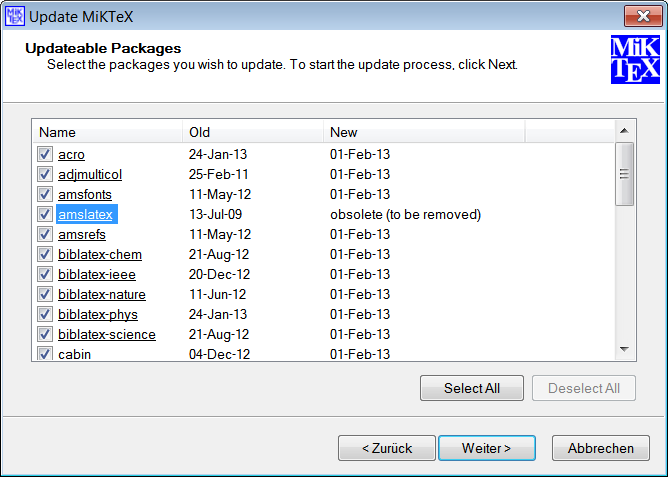
\includegraphics[width=8cm]{images/miktex-update}

    \MiKTeX\ Updater
  \end{center}\end{minipage}
\end{Frame}

\begin{Frame}{Pakete installieren und aktualisieren}{Linux}
  \begin{minipage}{\textwidth}\begin{center}
    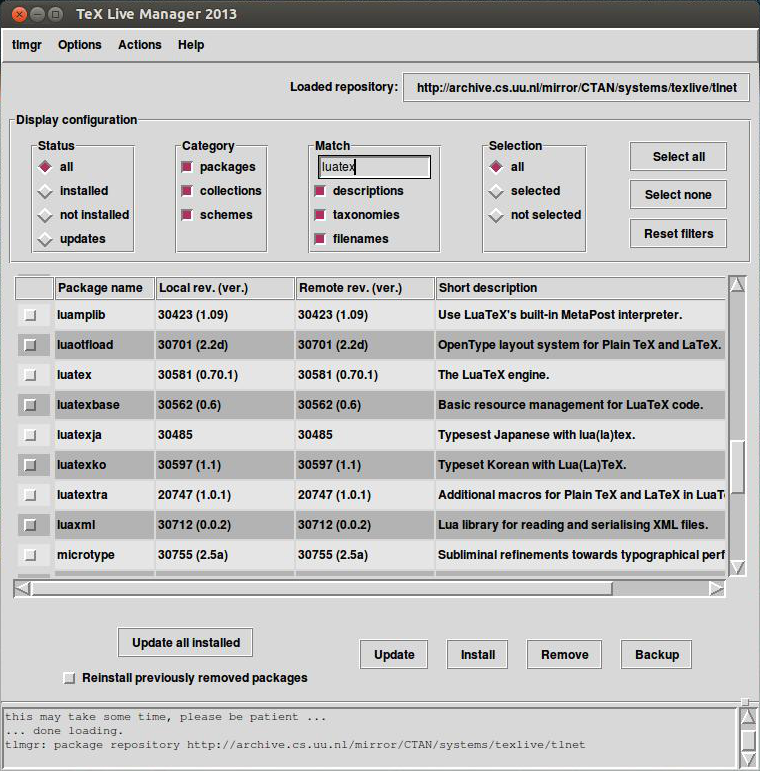
\includegraphics[width=7cm]{images/texlive-update}

    \TeX\ Live Manager
  \end{center}\end{minipage}
\end{Frame}

\begin{Frame}{Pakete installieren und aktualisieren}{Mac}
  \begin{minipage}{\textwidth}\begin{center}
    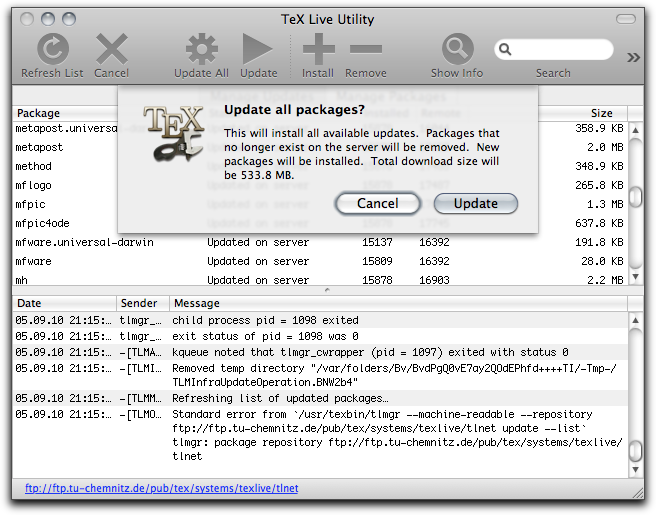
\includegraphics[width=8cm]{images/mactex-update}

    \TeX\ Live Utiliy
  \end{center}\end{minipage}
\end{Frame}

\mode
<article>

\begin{Frame}[fragile]{\TeX-Live-Pakete unter Ubuntu/Debian}
  \begin{lstlisting}[gobble=4,language={},morekeywords={sudo,apt,get}]
    sudo apt-get install texlive \
      texlive-lang-german texlive-latex-extra
  \end{lstlisting}

  installiert die Pakete

  \begin{description}
    \item[texlive] vollständiges \TeX-System, 
    \item[texlive-lang-german] deutsche Sprachunterstützung und
    \item[texlive-latex-extra] viele zusätzliche \LaTeX-Pakete.
  \end{description}

  \begin{alertblock}{Manuelle Installation}
    \begin{itemize}
      \item manuelle Installation ist oft aktueller
      \item vor Ubuntu 12.10 nur \TeX\ Live 2009 verfügbar
      \item Paketmanagement mit Paket \texttt{texlive-dummy} austricksen
        (vgl. Anleitung von ubuntuusers)
    \end{itemize}
  \end{alertblock}
\end{Frame}

\mode
<all>


\subsection{Verwendung}

\begin{Frame}[fragile]{\LaTeX}
  \begin{itemize}
    \item Ein \LaTeX-Dokument ist ein \alert{reines Textdokument}.
    \item Das \LaTeX-Dokument enthält \alert{Inhalt und Struktur}.
    \item \LaTeX\ setzt den Inhalt und kümmert sich um \alert{gute Form}.
  \end{itemize}

  \xxx
  
  \begin{center}
    \begin{tikzpicture}[
        shorten <=5pt,
        shorten >=5pt
      ]
      \matrix[column sep=3em] {
        \node[text width=6em] (source) {
          \lstinputlisting[
              basicstyle=\ttfamily\fontsize{4}{4}\selectfont,
              linerange={1-1,12-27}
            ]{demo/example.tex}
        };
        &
        \node[inner sep=0pt] (latex)
          {\rmfamily\Large\bfseries\LaTeX};
        &
        \node[draw=maincolor, thick] (pdf) {
          \includegraphics[width=6em]{demo/example.pdf}
        };\\
        \node {\shortstack{Inhalt \&\\ Struktur}};
        & & 
        \node {\shortstack{formatiertes\\Dokument}};\\
      };
      \path[very thick, ->]
        (source) edge (latex)
        (latex) edge (pdf);
    \end{tikzpicture}
  \end{center}
\end{Frame}

\begin{Frame}[fragile,t]{Ein \LaTeX-Dokument}
  \inhead{\texttt{hello.tex}}
  \lstinputlisting[linerange={1-2,5-8}]{demo/hello.tex}

  \pause
  \xxx

  \inhead{Kompilieren}
  \begin{lstlisting}[language={},morekeywords={pdflatex},gobble=4]
    pdflatex hello
  \end{lstlisting}

  \pause
  \xxx

  \inhead{\texttt{hello.pdf}}
  \begin{center}
    \includegraphics[width=4in]{demo/hello.pdf}
  \end{center}
\end{Frame}

\begin{Frame}{Editoren und IDEs}
  \begin{Block}{Editoren}
    \begin{itemize}
      \item Notepad++ (Windows)
      \item GEdit (Linux)
      \item Sublime Text (Windows, Linux, Mac)
    \end{itemize}
  \end{Block}

  \pause

  \begin{Block}{IDEs}
    \begin{itemize}
      \item \TeX works
        \begin{itemize}
          \item in \MiKTeX, \TeX\ Live und Mac\TeX\ enthalten
        \end{itemize}
      \item \TeX Shop
        \begin{itemize}
          \item in Mac\TeX\ enthalten
        \end{itemize}
      \item Kile (Linux)
      %\item Texmaker (Windows, Linux, Mac)
      \item TeXstudio (Windows, Linux, Mac)
      %\item \TeX nicCenter (Windows)
    \end{itemize}
  \end{Block}
\end{Frame}


\beamersection{\LaTeX\ verwenden}

\begin{Frame}[fragile]{Leerzeichen und Umbrüche}
  \begin{itemize}
    \item Zusätzliche \alert{Leerzeichen} werden ignoriert.
    \item \alert{Zeilenumbrüche} werden ignoriert.
  \end{itemize}

  \xxx

  \begin{exampleblock}{Absatz}
    \begin{itemize}
      \item \alert{Absatz}: leere Zeile in der Eingabe
      \item Aussehen variiert je nach Einstellungen.
    \end{itemize}
  \end{exampleblock}

  \xxx

  \begin{alertblock}{Manueller Zeilenumbruch}
    \begin{itemize}
      \item \alert{Zeilenumbruch}: \lstinline-\\-
      \item Ist \alert{hässlich} und \alert{stört} den Lesefluss.
    \end{itemize}
  \end{alertblock}
\end{Frame}

\subsection{Befehle und Umgebungen}

\begin{Frame}[fragile]{Befehle}{Hervorheben von Text}
  \begin{itemize}
    \item \lstinline-\emph{hervor}- hebt Text \emph{hervor}
    \item \lstinline-\textbf{fett}- macht Text \textbf{fett}
  \end{itemize}

  \xxx

  \begin{lstlisting}[gobble=4]
    Vorm \textbf{Senatsgebäude} stieß Caesar
    auf den \emph{Seher Spurinna}.
  \end{lstlisting}

  Vorm \textbf{Senatsgebäude} stieß Caesar
    auf den \emph{Seher Spurinna}.

  \xxx\pause

  \inhead{Weitere Auszeichnungen}
  \begin{itemize}
    \item \lstinline-\texttt{nichtproportional}- setzt \texttt{nichtproportional}
    \item \lstinline-\textsc{in Kapitälchen}- setzt \textsc{in Kapitälchen}
    \item \ldots
  \end{itemize}
\end{Frame}

\begin{Frame}[fragile]{komplexere Befehle}{Farbe und Fußnote}
  \inhead{Mehrere Argumente}
  \begin{lstlisting}[gobble=4]
    \textcolor{red}{Rosen} sind rot,
    \textcolor{blue}{Veilchen} sind blau.
  \end{lstlisting}
  \textcolor{red}{Rosen} sind rot,
  \textcolor{blue}{Veilchen} sind blau.
  
  \xxx\pause

  \inhead{Optionale Parameter}
  \begin{onlyenv}<presentation:1-2| article:0>
    \begin{lstlisting}[gobble=6]
      Vorm Senatsgebäude stieß Caesar\footnote{
        geb. 13. Juli 100 v. Chr. in Rom;
        gest. 15. März 44 v. Chr. ebenda}
      auf den Seher Spurinna.
    \end{lstlisting}
  \end{onlyenv}
  \begin{onlyenv}<3>
    \begin{lstlisting}[gobble=6]
      Vorm Senatsgebäude stieß Caesar\footnote[42]{
        geb. 13. Juli 100 v. Chr. in Rom;
        gest. 15. März 44 v. Chr. ebenda}
      auf den Seher Spurinna.
    \end{lstlisting}
  \end{onlyenv}
  \begin{minipage}{\textwidth}
    \renewcommand{\thempfootnote}{\arabic{mpfootnote}}
    Vorm Senatsgebäude stieß
      Caesar\alt<presentation:1-2| article:0>{\footnote{
        geb. 13. Juli 100 v. Chr. in Rom;
        gest. 15. März 44 v. Chr. ebenda}}
        {\footnote[42]{
        geb. 13. Juli 100 v. Chr. in Rom;
        gest. 15. März 44 v. Chr. ebenda}}
      auf den Seher Spurinna.
  \end{minipage}
\end{Frame}

\begin{Frame}[fragile]{Befehle}{Merkmale}
  \begin{itemize}
    \item Befehle beginnen mit einem Backslash.\newline
      z.\,B. \lstinline-\emph-
    \item Parameter stehen in geschweiften Klammern.\newline
      z.\,B. \lstinline-\emph{hervor}-
    \item Weitere Parameter folgen in geschweiften Klammern.\newline
      z.\,B. \lstinline-\textcolor{red}{Rosen}-
    \item Optionale Paramter stehen in eckigen Klammern.\newline
      z.\,B. \lstinline-\footnote[42]{geb.}-
  \end{itemize}
\end{Frame}

\begin{Frame}[fragile]{Umgebungen}{Zentrieren}
  \begin{lstlisting}[gobble=4]
    Normaler Text im Blocksatz.

    \begin{center}
      Ich bin zentriert.
    \end{center}
  \end{lstlisting}

  \xxx

  \begin{minipage}{\textwidth}
    Normaler Text im Blocksatz.
    \lorem
  \end{minipage}  

  \begin{center}
    Ich bin zentriert. \lorem
  \end{center}

  \pause

  \inhead{Weitere Ausrichtungen}
  \begin{itemize}
    \item \lstinline-flushleft- erzeugt \alert{linksbündigen Flattersatz}.
    \item \lstinline-flushright- erzeugt \alert{rechtsbündigen Flattersatz}.
  \end{itemize}
\end{Frame}

\begin{Frame}[fragile]{Umgebungen}{Zitieren}
  \begin{lstlisting}[gobble=4]
    \begin{quote}
      Ich bin ein Zitat.
    \end{quote}
  \end{lstlisting}

  \xxx

  \begin{minipage}{\textwidth}
    Normaler Text im Blocksatz.
    \lorem
  \end{minipage}

  \begin{quote}
    Ich bin ein Zitat. \lorem
  \end{quote}

  \pause

  \inhead{Weitere Zitationen}
  \begin{itemize}
    \item \lstinline-quote- für \alert{kurze Zitate}.
    \item \lstinline-quotation- für \alert{lange Zitate} über mehrere Absätze.
    \item \lstinline-verse- für Zitate von \alert{Gedichten} u.\,ä.
  \end{itemize}
\end{Frame}

\begin{Frame}[fragile]{Umgebungen}
  \begin{itemize}
    \item Umgebungen beginnen mit \lstinline-\begin-\newline
      z.\,B. \lstinline-\begin{center}-
    \item und enden mit \lstinline-\end-.\newline
      z.\,B. \lstinline-\end{center}-
    \item Erster Parameter ist jeweils der Name der Umgebung.
    \item Weitere Parameter nur nach \lstinline-\begin-.\newline
      z.\,B. \lstinline-\begin{tabular}{ll}-
  \end{itemize}
\end{Frame}

\subsection{Aufbau und Präambel}

\mode
<article>

\begin{Frame}[fragile]{Aufbau eines Dokuments}
  \begin{lstlisting}[gobble=4]
    % Dokumentenklasse
    \documentclass{scrartcl}

    % Präambel: Pakete laden
    \usepackage[ngerman]{babel}
    \usepackage[utf8]{inputenc}
    \usepackage[T1]{fontenc}

    % Präambel: Einstellungen
    \KOMAoptions{%
      parskip=full,%
      fontsize=12pt}

    % Dokumentenkörper
    \begin{document}
      Franz jagt im komplett
      verwahrlosten Taxi quer
      durch Bayern.
    \end{document}
  \end{lstlisting}
\end{Frame}

\mode
<presentation>

\begin{Frame}[fragile]{Aufbau eines Dokuments}
  \begin{tikzpicture}[%
      auto,
      every edge/.style={
        draw,
        decorate,
        decoration=brace,
        very thick
      }
    ]
    \node[text width=\textwidth, anchor=south] (tex) {
      \begin{lstlisting}[gobble=8]
        \documentclass{scrartcl}

        \usepackage[ngerman]{babel}
        \usepackage[utf8]{inputenc}
        \usepackage[T1]{fontenc}

        \KOMAoptions{%
          parskip=full,%
          fontsize=12pt}

        \begin{document}
          Franz jagt im komplett
          verwahrlosten Taxi quer
          durch Bayern.
        \end{document}
      \end{lstlisting}
    };

    \pause
    \draw
      (1,7.6) edge node {Dokumentenklasse} (1,7.2);
    \pause
    \draw
      (1,6.6) edge node {\shortstack{Pakete\\laden}} (1,5.3);
    \pause
    \draw
      (0,4.7) edge node {Einstellungen} (0,3.5);
    \pause
    \draw
      (3,6.6) edge node {Präambel} (3,3.5);
    \pause
    \draw
      (1,2.6) edge node {Dokumentenkörper} (1,.9);
  \end{tikzpicture}
\end{Frame}

\mode
<all>

\begin{Frame}[fragile]{Dokumentenklassen}
  \lstinline-\documentclass{scrartcl}-\newline
  kurzer Artikel

  \xxx

  \lstinline-\documentclass{scrreprt}-\newline
  Bericht mit Titelseite und Kapiteln

  \xxx

  \lstinline-\documentclass{scrbook}-\newline
  doppelseitiges Buch mit Teilen, Kapiteln und Kopfzeile

  \xxx

  \begin{alertblock}{amerikanische Dokumentenklassen}
    Wir verwenden die deutschen Dokumentenklassen aus KOMA-Script statt der 
    amerikanischen \lstinline-article-, \lstinline-report- und \lstinline-book-.
  \end{alertblock}
\end{Frame}

\mode
<article>

\begin{Frame}[fragile]{Präambel: KOMA-Script-Optionen}
  \begin{lstlisting}[gobble=4]
    \KOMAoptions{
      parskip=full,
      % full - Absätze haben großen Abstand
      % half - Absätze haben kleinen Abstand
      % off  - Absätze haben Einzug (default)
      fontsize=12pt,
      % Grundschriftgröße (10pt default)
      headings=small,
      % small  - kleine Überschriften
      % normal - normale Überschriften (default)
      % big    - große Überschriften
      paper=a5,
      % Papierformat (a4 default)
      pagesize=auto
      % Papierformat auch für PDF verwenden
    }
  \end{lstlisting}
\end{Frame}

\mode
<all>

\begin{Frame}[fragile]{Präambel: Pakete}
  \lstset{
    backgroundcolor={},
    frame=no,
    gobble=4,
    aboveskip=3ex,
    belowskip=0pt
  }
  \begin{lstlisting}
    \usepackage[ngerman]{babel}
  \end{lstlisting}
  deutsche Silbentrennung und deutsche Übersetzung
  \begin{lstlisting}
    \usepackage[utf8]{inputenc}
  \end{lstlisting}
  UTF-8 als Zeichenkodierung verwenden
  \begin{lstlisting}
    \usepackage[T1]{fontenc}
  \end{lstlisting}
  westeuropäische Schriftkodierung verwenden
  \begin{lstlisting}
    \usepackage{lmodern}
  \end{lstlisting}
  schönere Schriftarten verwenden
  \begin{lstlisting}
    \usepackage[breaklinks=true]{hyperref}
  \end{lstlisting}
  bessere Unterstützung der PDF-Ausgabe
  \begin{onlyenv}<article>
    \begin{lstlisting}[gobble=6]
      \usepackage[breaklinks=true, pdfborder={0 0 0},
                  pdfhighlight={/N}]{hyperref}
    \end{lstlisting}
    noch bessere Unterstützung der PDF-Ausgabe
  \end{onlyenv}
\end{Frame}

\subsection{Gliederung und Titel}

\begin{Frame}[fragile,t]{Gliederung}
  \xxx

  \begin{onlyenv}<1>
    \begin{Block}{Strukturbefehle}
      \begin{itemize}
        \item \lstinline-\part{name}- für Teile (nur in Büchern)
        \item \lstinline-\chapter{name}- für Kapitel (nicht in Artikeln)
        \item \lstinline-\section{name}- für Abschnitte
        \item \lstinline-\subsection{name}- für Unterabschnitte
      \end{itemize}
    \end{Block}
  \end{onlyenv}

  \begin{onlyenv}<2-3>
    \begin{Block}{Strukturbefehle}
      \begin{itemize}
        \item \lstinline-\part[kurz]{name}- für Teile (nur in Büchern)
        \item \lstinline-\chapter[kurz]{name}- für Kapitel (nicht in Artikeln)
        \item \lstinline-\section[kurz]{name}- für Abschnitte
        \item \lstinline-\subsection[kurz]{name}- für Unterabschnitte
      \end{itemize}
    \end{Block}

    Optionaler Parameter setzt Kurztitel für Inhaltsverzeichnis.
  \end{onlyenv}

  \begin{onlyenv}<4>
    \begin{Block}{Strukturbefehle}
      \begin{itemize}
        \item \lstinline-\part*{name}- für Teile (nur in Büchern)
        \item \lstinline-\chapter*{name}- für Kapitel (nicht in Artikeln)
        \item \lstinline-\section*{name}- für Abschnitte
        \item \lstinline-\subsection*{name}- für Unterabschnitte
      \end{itemize}
    \end{Block}

    Variante mit \texttt{*} erscheint nicht im Inhaltsverzeichnis
  \end{onlyenv}

  \xxx

  \begin{onlyenv}<3->
    \begin{lstlisting}[gobble=6]
      \tableofcontents
    \end{lstlisting}
    setzt das zugehörige Inhaltsverzeichnis.
  \end{onlyenv}
\end{Frame}

\begin{Frame}[t,fragile]{Titelseite}{Automatisch}
  \begin{Block}{In der Präambel}
    \lstinputlisting[firstline=13, lastline=16, style=block]{demo/maketitle.tex}
  \end{Block}

  \begin{Block}{Am Anfang des Dokuments}
    \begin{lstlisting}[gobble=6,style=block]
      \maketitle
    \end{lstlisting}
  \end{Block}

  \hfill \includegraphics[width=8cm]{demo/maketitle} \hfill
\end{Frame}

\begin{Frame}[fragile]{Titelseite}{Manuell}
  \lstinputlisting[firstline=15, lastline=22]{demo/titlepage.tex}

  \hfill \includegraphics[width=8cm]{demo/titlepage} \hfill
\end{Frame}

\subsection{Detailtypographie}

\begin{Frame}[fragile]{Sonderzeichen}
  \begin{zebratabular}{llll}
    \headerrow Name & Symbol & \LaTeX-Code\\
    Backslash & \textbackslash & \lstinline-\textbackslash-\\
    geschweifte Klammern & \{, \} & \lstinline-\{-, \lstinline-\}-\\
    Doppelkreuz & \# & \lstinline-\#-\\
    Dollarzeichen & \$ & \lstinline-\$-\\
    Unterstrich & \_ & \lstinline-\_-\\
    Zirkumflex & \textasciicircum & \lstinline-\textasciicircum-\\
    Kaufmanns-Und & \& & \lstinline-\&-\\
    Prozentzeichen & \% & \texttt{\textbackslash \%}\\
    Tilde & \textasciitilde & \lstinline-\textasciitilde-
  \end{zebratabular}
\end{Frame}

\mode
<article>

Spitze Klammern < und > haben in bestimmten Kontexten eine spezielle Bedeutung. Deswegen können sie auch als \lstinline-\textless- und \lstinline-\textgreater- eingegeben werden. Durch die Verwendung des Pakets \lstinline-inputenc- können sie aber auch direkt eingegeben werden. Genauso kann das Paragraphenzeichen § auch als \lstinline-\S- eingegeben werden.

Wir werden später sehen, dass \LaTeX\ einen eigenen Mathe-Modus hat. Einige Zeichen werden in diesem Modus anders behandelt. Insbesondere die Kommandos, die mit \lstinline-\text- beginnen, sollten in diesem Modus mit Vorsicht verwendet werden. Statt \lstinline-\textbackslash- steht hier der Befehl \lstinline-\backslash- zur Verfügung, tatt \lstinline-\textasciitilde- sollte man \lstinline-\sim- verwenden und für \lstinline-\textasciicircum- existiert hier kein guter Ersatz.

\mode
<all>

\begin{Frame}[fragile]{Binde- und sonstige Striche}
  \begin{looseitemize}
    \item Bindestrich
      \begin{lstlisting}[gobble=8]
        SOS-Ruf
      \end{lstlisting}
      SOS-Ruf
    \item deutscher Gedankenstrich mit Leerzeichen
      \begin{lstlisting}[gobble=8]
        Er kam -- und ging gleich wieder.
      \end{lstlisting}
      Er kam -- und ging gleich wieder.
    \item britischer Gedankenstrich ohne Leerzeichen
      \begin{lstlisting}[gobble=8]
        He came---and went.
      \end{lstlisting}
      He came---and went.
  \end{looseitemize}
\end{Frame}

\begin{Frame}[fragile]{Leerzeichen}
  \begin{looseitemize}
    \item normales flexibles Leerzeichen
      \begin{lstlisting}[gobble=8]
        Leerzeichen stehen zwischen Worten.
      \end{lstlisting}
    \item geschütztes flexibles Leerzeichen
      \begin{lstlisting}[gobble=8]
        Hier~wird~nicht~umgebrochen.
      \end{lstlisting}
    \item Abstand in der Breite eines Ms (1~quad)
      \begin{lstlisting}[gobble=8]
        Ein Satz.\quad Noch ein Satz.\qquad Ende.
      \end{lstlisting}
      Ein Satz.\quad Noch ein Satz. \qquad Ende.
  \end{looseitemize}
\end{Frame}

\begin{Frame}[fragile]{Abkürzungen}
  \begin{Block}{Mehrgliedrige Abkürzungen}
    \begin{itemize}
      \item mehrgliedrige Abkürzungen eng zusammen setzen
      \item einen 3/18 quad Abstand verwenden
        \begin{lstlisting}[gobble=10]
          Abkürzungen, z.\,B. diese
        \end{lstlisting}
        Abkürzungen, z.\,B. diese
    \end{itemize}
  \end{Block}
  
  \begin{Block}{Umbrüche vermeiden}
    \begin{itemize}
      \item Zusammenhängende Kürzel nicht trennen
      \item Maß- und Währungszeichen nicht von der Zahl trennen
      \item geschütztes Leerzeichen \lstinline-~- verwenden
        \begin{lstlisting}[gobble=10]
          Seite~5, 4~km, S.~5~ff.
        \end{lstlisting}
        Seite~5, 4~km, S.~5~ff.
    \end{itemize}
  \end{Block}
\end{Frame}

\begin{Frame}[fragile]{Anführungszeichen}
  \begin{alertblock}{Verwendung}
    Anführungszeichen sind nur für \alert{wörtliche Zitate}.
  \end{alertblock}
  
  \begin{Block}{In der Präambel}
    \begin{lstlisting}[gobble=6,style=block]
      \usepackage[german=guillemets]{csquotes}
      % oder german=quotes
      % oder english=british oder english=american
    \end{lstlisting}
  \end{Block}

  \begin{lstlisting}[gobble=4]
    Hans sagt: \enquote{Er habe \enquote{Franz'
    Auto!} gerufen.}
  \end{lstlisting}

  Hans sagt: \enquote{Er habe \enquote{Franz' Auto!} gerufen.}
\end{Frame}

\mode
<article>

\begin{Frame}[fragile]{Schriftgröße}
  \begin{itemize}
    \item \lstinline-{\tiny winzig}- setzt {\tiny winzig}
    \item \lstinline-{\scriptsize in Indexgröße}- setzt {\scriptsize in Indexgröße}
    \item \lstinline-{\footnotesize in Fußzeilengröße}-\\ setzt {\footnotesize in Fußzeilengröße}
    \item \lstinline-{\small klein}- setzt {\small klein}
    \item \lstinline-{\normalsize in Normalgröße}-\\ setzt {\normalsize in Normalgröße}
    \item \lstinline-{\large groß}- setzt {\large groß}
    \item \lstinline-{\Large größer}- setzt {\Large größer}
    \item \lstinline-{\LARGE am größten}- setzt {\LARGE am größten}
    \item \lstinline-{\huge riesig}- setzt {\huge riesig}
    \item \lstinline-{\Huge riesiger}- setzt {\Huge riesiger}
  \end{itemize}
\end{Frame}

\mode
<all>


\beamersection{Elemente}

\subsection{Farbe}

\begin{Frame}[fragile]{Farben verwenden}
  \begin{Block}{In der Präambel}
    \begin{lstlisting}[gobble=6,style=block]
      \usepackage{xcolor}
    \end{lstlisting}
  \end{Block}

  \xxx

  \begin{lstlisting}[gobble=4]
    In diesem \colorbox{orange}{Text} sind
    \textcolor{orange}{Worte} hervorgehoben.
  \end{lstlisting}

  In diesem \colorbox{orange}{Text} sind
  \textcolor{orange}{Worte} hervorgehoben.
\end{Frame}

\begin{Frame}{Vorhandene Farben}
  \colorsample{red}\newline
  \colorsample{green}\newline
  \colorsample{blue}\newline
  \colorsample{cyan}\newline
  \colorsample{magenta}\newline
  \colorsample{yellow}

  \xxx

  \colorsample{black}\newline
  \colorsample{white}\newline
  \colorsample{darkgray}\newline
  \colorsample{gray}\newline
  \colorsample{lightgray}
\end{Frame}

\begin{Frame}{Farben mischen}
  \colorsample{red}\newline
  \pause
  \colorsample{red!75}\newline
  \pause
  \colorsample{red!75!green}\newline
  \pause
  \colorsample{red!75!green!50}\newline
  \pause
  \colorsample{red!75!green!50!blue}\newline
  \pause
  \colorsample{red!75!green!50!blue!25}\newline
  \pause
  \colorsample{red!75!green!50!blue!25!gray}
  \pause

  \xxx

  \colorsample{-red}\newline
  \colorsample{-red!75}\newline
  \colorsample{-red!75!green}\newline
  \colorsample{-red!75!green!50}\newline
  \colorsample{-red!75!green!50!blue}\newline
  \colorsample{-red!75!green!50!blue!25}\newline
  \colorsample{-red!75!green!50!blue!25!gray}
\end{Frame}

\subsection{Formeln}

\begin{Frame}[fragile]{Formelsatz in Matheumgebungen}
  \begin{Block}{In der Präambel}
    \begin{lstlisting}[gobble=6,style=block]
      \usepackage{amsmath}
      \usepackage{amssymb}
    \end{lstlisting}
  \end{Block}
  
  \begin{looseitemize}
    \item in normalen Text: \lstinline-$x^y$- erzeugt $x^y$
    \item abgesetzt: \lstinline-\[ x^3 \]- erzeugt
      \[ x^3 \]
    \item mehrzeilig: \lstinline-align-, ausgerichtet an \lstinline-&-, neue Zeile mit \lstinline-\\- 
      \begin{lstlisting}[gobble=8]
        \begin{align} % ohne Nummerierung mit align*
          f(x) &= x^3 \\
               &= x \cdot x \cdot x
        \end{align}
      \end{lstlisting}
      \begin{align}
        f(x) &= x^3 \\
             &= x \cdot x \cdot x
      \end{align}
  \end{looseitemize}
\end{Frame}

\begin{Frame}[fragile]{Beispiele zum Formelsatz}
  \only<presentation>{\lstset{aboveskip=3pt,belowskip=3pt}}

  \newcommand{\mathexample}[1]{\alt<presentation>{%
    $\displaystyle\displaystyle#1$%
  }{%
    \[ #1 \]
  }}

  \begin{columns}
    \column{5cm}
      \begin{lstlisting}[gobble=8]
        \alpha^{22} + \beta_{12}
          = \gamma^2_a
      \end{lstlisting}

    \column{4cm}
      \mathexample{\alpha^{22} + \beta_{12} = \gamma^2_a}
  \end{columns}

  \pause

  \begin{columns}
    \column{5cm}
      \begin{lstlisting}[gobble=8]
        \sum_{i=1}^{n} i =
          \frac{n (n+1)}{2}
      \end{lstlisting}

    \column{4cm}
      \mathexample{\sum_{i=1}^n i = \frac{n (n+1)}{2}}
  \end{columns}

  \pause

  \begin{columns}
    \column{5cm}
      \begin{lstlisting}[gobble=8]
        \sqrt{x^{4}} = x^{2}
      \end{lstlisting}

    \column{4cm}
      \mathexample{\sqrt{x^4} = x^2}
  \end{columns}

  \pause

  \begin{columns}
    \column{5cm}
      \begin{lstlisting}[gobble=8]
        \lim_{n\to\infty}
          \frac{1}{n^{2}} = 0
      \end{lstlisting}

    \column{4cm}
      \mathexample{\lim_{n\to\infty} \frac{1}{n^2} = 0}
  \end{columns}
  
  \pause

  \begin{columns}
    \column{5cm}
      \begin{lstlisting}[gobble=8]
        \int_{-1}^{2}
          x\,\mathrm{d}x = \left[
            \frac{1}{2}x^{2}
          \right]_{1}^{2}
      \end{lstlisting}

    \column{4cm}
      \mathexample{\int_{-1}^{2} x\,\mathrm{d}x=\left[ \frac{1}{2}x^2 \right]_1^2}
  \end{columns}
\end{Frame}

\begin{Frame}[fragile]{Dezimaltrennzeichen in Zahlen}
  \begin{Block}{Amerikanisches Format}
    \begin{lstlisting}[gobble=6,style=block]
      \[ 23,456.78 - 23\,456.78 + 23456.78 \]
    \end{lstlisting}

    \[ 23,456.78 - 23\,456.78 + 23456.78 \]
  \end{Block}

  \xxx

  \begin{Block}{Deutsches Format}
    \begin{lstlisting}[gobble=6,style=block]
      \[ 23.456{,}78 - 23\,456{,}78 + 23456{,}78 \]
    \end{lstlisting}

    \[ 23.456{,}78 - 23\,456{,}78 + 23456{,}78 \]
  \end{Block}
\end{Frame}

\mode
<article>

\begin{Block}{Minuszeichen als binärer und unärer Operator}
  \begin{lstlisting}[gobble=4]
    $2-4=-2$ (nicht -2)
  \end{lstlisting}
  $2-4=-2$ (nicht -2)
  \only<article>{
    \newline Als binärer Operator wird das Minuszeichen mit einem kleinen Abstand gesetzt.
    Als unärer Operator wird das Minuszeichen als Vorzeichen ohne Abstand gesetzt.
    \LaTeX\ übernimmt dies automatisch.
  }
\end{Block}

\mode
<all>

\subsection{Listen und Tabellen}

\begin{Frame}[fragile]{Listen}
  \begin{columns}
    \column{5cm}
      \begin{lstlisting}[gobble=8]
        \begin{itemize}
          \item Apfel
            \begin{itemize}
              \item Elstar
              \item Braeburn
            \end{itemize}
          \item Birne
        \end{itemize}
      \end{lstlisting}
    \column{4cm}
      \begin{itemize}
        \item Apfel
          \begin{itemize}
            \item Elstar
            \item Braeburn
          \end{itemize}
        \item Birne
      \end{itemize}
  \end{columns}
  
  \begin{columns}
    \column{5cm}
      \begin{lstlisting}[gobble=8]
        \begin{enumerate}
          \item Begrüßung
          \item Anträge
          \item Verabschiedung
        \end{enumerate}
      \end{lstlisting}
    \column{4cm}
      \begin{enumerate}
        \item Begrüßung
        \item Anträge
        \item Verabschiedung
      \end{enumerate}
  \end{columns}
\end{Frame}

\begin{Frame}[fragile]{Listen}{Definitionslisten}
  \begin{lstlisting}[gobble=4]
    \begin{description}
      \item[Das Schlagwort] steht am Anfang
        einer Zeile und wird hervorgehoben,
        während der zugehörige
      \item[Text] dahinter in normaler
        Schrift erscheint.
    \end{description}
  \end{lstlisting}

  \begin{description}
    \item[Das Schlagwort] steht am Anfang einer Zeile und wird
      hervorgehoben, während der zugehörige
    \item[Text] dahinter in normaler Schrift erscheint.
  \end{description}
\end{Frame}

\begin{Frame}[fragile]{Tabellen}
  \begin{lstlisting}[gobble=4]
    \begin{tabular}{l|lr}
      \textbf{Jahr} & \textbf{Prozessor} &
          \textbf{MHz} \\
      \hline
      1975 & 6502 (C64) & 1 \\
      1985 & 80386 & 16 \\
      2005 & Pentium 4 & 2\,800 \\
      2030 & Phoenix 3 & 7\,320\,000
    \end{tabular}
  \end{lstlisting}

  \begin{center}
    \begin{tabular}{l|lr}
      \textbf{Jahr} & \textbf{Prozessor} &
          \textbf{MHz} \\
      \hline
      1975 & 6502 (C64) & 1 \\
      1985 & 80386 & 16 \\
      2005 & Pentium 4 & 2\,800 \\
      2030 & Phoenix 3 & 7\,320\,000
    \end{tabular}
  \end{center}
\end{Frame}

\begin{Frame}[fragile]{Zebratabellen}
  \begin{Block}{Option in der Präambel setzen}
    \begin{lstlisting}[gobble=6,style=block]
      \usepackage[table]{xcolor}
    \end{lstlisting}
  \end{Block}

  \begin{lstlisting}[gobble=4]
    \rowcolors{1}{orange!25}{orange!5}
    \begin{tabular}{llr}
      \rowcolor{orange!50}
      Jahr & Prozessor & MHz \\
      1975 & 6502 (C64) & 1 \\
      1985 & 80386 & 16 \\
      2005 & Pentium 4 & 2\,800
    \end{tabular}
  \end{lstlisting}

  \rowcolors{1}{orange!25}{orange!5}
  \begin{center}  
    \begin{tabular}{llr}
      \rowcolor{orange!50}
      Jahr & Prozessor & MHz \\
      1975 & 6502 (C64) & 1 \\
      1985 & 80386 & 16 \\
      2005 & Pentium 4 & 2\,800
    \end{tabular}
  \end{center}
\end{Frame}

\begin{frame}[fragile]{Fließumgebungen}
  \inhead{Fließumgebungen}
  \begin{itemize}
    \item werden automatisch im Dokument positioniert.
    \item erhalten Nummerierung und Beschriftung.
    \item können referenziert werden.
    \item werden in Verzeichnisse aufgenommen.
  \end{itemize}

  \begin{lstlisting}[gobble=4]
    \begin{table} % Fließumgebung
      \begin{tabular}{ll} % eigentliche Tabelle
        Schafgarbe & gelb \\
        Ochsenzunge & violett
      \end{tabular}
      \caption{Färberpflanzen} % Beschriftung
    \end{table}
  \end{lstlisting}
\end{frame}

\begin{Frame}[fragile]{Positionierungshinweise}
  \begin{lstlisting}[gobble=4]
    \begin{table}[htb]
      \begin{tabular}{ll}
        % ...
      \end{tabular}
      \caption{Färberpflanzen}
    \end{table}
  \end{lstlisting}

  \xxx

  Element platzieren
  
  \begin{tabular}{lr@{ }l}
    & \lstinline-h- & an Position im Quelltext \\
    & \lstinline-b- & am Ende einer Seite \\
    & \lstinline-t- & am Anfang einer Seite \\
    & \lstinline-p- & auf einer eigenen Abbildungsseite \\
    & \lstinline-!- & \LaTeX s Bewertung der Platzierung abschalten
  \end{tabular}
\end{Frame}

\subsection{Abbildungen und Verweise}

\begin{Frame}[fragile]{Grafiken}
  \begin{Block}{In der Präambel}
    \begin{lstlisting}[gobble=6,style=block]
      \usepackage{graphicx}
    \end{lstlisting}
  \end{Block}

  \xxx

  \begin{columns}
    \column{5cm}
      \begin{lstlisting}[gobble=8]
        \includegraphics%
          [width=3.5cm]{miktex}
      \end{lstlisting}
    \column{4cm}
      
\includegraphics[width=3.5cm]{images/miktex}
  \end{columns}
\end{Frame}

\mode
<article>

\begin{Block}{Dateitypen}
  Bei der Verwendung von \pdfTeX\ können Grafikdateien in den Formaten PDF, JPG und PNG verwendet werden.
  Soll das Dokument mit \TeX\ kompiliert werden, muss die Grafik als EPS-Datei vorliegen. Aus diesem Grund
  wird die Grafikdatei häufig ohne Dateierweiterung angegeben, sodass die für den jeweiligen Fall am besten
  geeignete Datei automatisch verwendet wird.

  Leider gibt es keine Möglichkeit, SVG-Dateien direkt zu verwenden. Diese müssen vorher in PDF bwz. EPS konvertiert werden. Da beide Formate Vektorgrafiken unterstützen gehen bei dieser Konvertierung keine Informationen velohren.
\end{Block}

\mode
<all>

\begin{Frame}[fragile]{Grafiken rotieren und zuschneiden}
  \begin{columns}
    \column{5cm}
      \begin{lstlisting}[gobble=8]
        \includegraphics%
          [width=3.5cm,%
           angle=20]{miktex}
      \end{lstlisting}
    \column{4cm}
      
\includegraphics[width=3.5cm,angle=20]{images/miktex}
  \end{columns}

  \xxx

  \begin{columns}
    \column{5cm}
      \begin{lstlisting}[gobble=8]
        \includegraphics%
          [width=3.5cm,trim=%
           3cm 5mm 4cm 12mm,%
           clip=true]{miktex}
      \end{lstlisting}
    \column{4cm}
      
\includegraphics[width=3.5cm,trim=3cm 5mm 4cm 12mm,clip=true]{images/miktex}
  \end{columns}

  schneidet links 3\,cm, unten 5\,mm,\\ rechts 4\,cm und oben 12\,mm ab
\end{Frame}

\begin{frame}[fragile]{Fließumgebungen}
  Fließumgebungen für Abbildungen funktionieren\\
  wie Fließumgebungen für Tabellen.

  \begin{lstlisting}[gobble=4]
    \begin{figure} % Fließumgebung
      % Grafik zentrieren
      \centering
      % eigentliche Grafik
      
\includegraphics[width=3.5cm]{miktex}
      % Beschriftung
      \caption{Färberpflanzen}
    \end{figure}
  \end{lstlisting}
\end{frame}

\begin{Frame}[fragile]{Verzeichnisse}
  \begin{Block}{Inhaltsverzeichnis}
    \begin{lstlisting}[gobble=6,style=block]
      \tableofcontents
    \end{lstlisting}
  \end{Block}

  \begin{Block}{Abbildungsverzeichnis}
    \begin{lstlisting}[gobble=6,style=block]
      \listoffigures
    \end{lstlisting}
  \end{Block}

  \begin{Block}{Tabellenverzeichnis}
    \begin{lstlisting}[gobble=6,style=block]
      \listoftables
    \end{lstlisting}
  \end{Block}

  \xxx

  \begin{alertblock}{Warnung}
    Welchen Nutzen haben Abbildungs- und Tabellenverzeichnis?
  \end{alertblock}
\end{Frame}

\begin{Frame}[fragile]{Verweise}
  \begin{looseitemize}
    \item \alert{Nach} Strukturbefehl oder Beschriftung Label angeben
      \begin{lstlisting}[gobble=8]
        \section{Verzeichnisse und Verweise}
        \label{sec-verweise}
        % ...
        \begin{figure} % oder auch table
          %...
          \caption{MiKTeX-Logo}
          \label{fig-miktex}
        \end{figure}
      \end{lstlisting}
     \item Label referenzieren
       \begin{lstlisting}[gobble=8]
         MiK\TeX-Logo auf \autoref{fig-miktex}
         in \autoref{sec-verweise}
       \end{lstlisting}
       \MiKTeX-Logo auf Abbildung 5 in Abschnitt 3.2
  \end{looseitemize}
\end{Frame}

\begin{Frame}{Mehrfach kompilieren hilft.}{Rerun to get cross-references right.}
  \begin{center}
    \begin{tikzpicture}[on grid, node distance=18mm and 35mm]
      \node[examplecolor] (tex) {\icon{TEX}};
      \uncover<2->{
        \node[right=of tex, font=\rmfamily\Large\bfseries]
          (pdfTeX1) {\pdfTeX};
      }
      \uncover<3>{
        \node[right=of pdfTeX1, pdficon] (pdf1) {\icon{PDF}};
        \node[below=of pdfTeX1, logicon, xshift=1cm] (log1) {\icon{LOG}};
      }
      \uncover<4->{
        \node[right=of pdfTeX1, pdficon!30] (pdf1) {\icon{PDF}};
        \node[below=of pdfTeX1, xshift=1cm, logicon!30] (log1) {\icon{LOG}};
      }
      \uncover<3->{
        \node[below=of pdfTeX1, xshift=-1cm, auxicon] (aux1) {\icon{AUX}};
      }
      \uncover<4->{
        \node[below=of aux1, xshift=1cm, font=\rmfamily\Large\bfseries]
          (pdfTeX2) {\pdfTeX};
      }
      \uncover<5>{
        \node[right=of pdfTeX2, pdficon] (pdf2) {\icon{PDF}};
        \node[below=of pdfTeX2, xshift=1cm, logicon] (log2) {\icon{LOG}};
        \node[below=of pdfTeX2, xshift=-1cm, auxicon] (aux2) {\icon{AUX}};
      }
      \only<2->{
        \draw[very thick]
          (tex) edge[->] (pdfTeX1);
      }
      \only<3->{
        \draw[very thick]
          (pdfTeX1) edge[->] (aux1);
      }
      \only<3>{
        \draw[very thick]
          (pdfTeX1) edge[->] (pdf1)
                    edge[->] (log1);
      }
      \only<4->{
        \draw[very thick, black!30]
          (pdfTeX1) edge[->] (pdf1)
                    edge[->] (log1);
      }
      \only<4->{
        \draw[very thick]
          (aux1) edge[->] (pdfTeX2);
        \draw[->, very thick] (tex.south) ++ (.2,0) |- (pdfTeX2);
      }
      \only<5->{
        \draw[very thick]
          (pdfTeX2) edge[->] (pdf2)
                    edge[->] (aux2)
                    edge[->] (log2);
      }
    \end{tikzpicture}
  \end{center}
\end{Frame}


\section*{Zusammenfassung}

\begin{frame}{Zusammenfassung}
  \begin{enumerate}
    \item Das \alert{\LaTeX-Dokument} enthält \alert{Inhalt und Struktur}.
    \item \LaTeX\ setzt ein druckfertiges \alert{PDF-Dokument} und kümmert sich dabei um die \alert{gute Form}.
    \item Es ist schwierig, \alert{neue Layouts} zu erzeugen.
    \item Ein \LaTeX-Dokument besteht aus \alert{Dokumentenklasse}, \alert{Präambel} und \alert{Dokumentenkörper}.
    \item Wir haben \alert{Auszeichnungen}, \alert{Formelsatz}, \alert{Listen}, \alert{Tabellen}, \alert{Abbildungen}, \alert{Verzeichnisse} und \alert{Verweise} kennen gelernt.
  \end{enumerate}
\end{frame}

\begin{Frame}[fragile]{Zum Weiterlesen}
  \begin{mybib}
    \bibitem{Wiki}
      Wikibooks contributors.
      \newblock \emph{\LaTeX\ Wikibook},
      \newblock \alt<presentation>{\href{http://en.wikibooks.org/wiki/LaTeX}{\texttt{en.wikibooks.org/LaTeX}}}{\url{http://en.wikibooks.org/wiki/LaTeX}}, November 2014
    \bibitem{basics_Kohm}
      Markus Kohm, Jens-Uwe-Morawski.
      \newblock \emph{KOMA-Script},
      \newblock \alt<presentation>{\href{http://mirrors.ctan.org/macros/latex/contrib/koma-script/doc/scrguide.pdf}{\texttt{scrguide.pdf}}}{\url{http://mirrors.ctan.org/macros/latex/contrib/koma-script/doc/scrguide.pdf}}, Dezember 2013.
  \end{mybib}
\end{Frame}

\begin{Frame}[fragile]{Zum weiteren Weiterlesen}
  \begin{mybib}
    \bibitem{basics_Kopka}
      Helmut Kopka.
      \newblock \emph{\LaTeX, Band 1: Einführung},
      \newblock Addison-Wesley, März 2002.
    \bibitem{basics_Braune}
      Klaus Braune, Joachim und Marion Lammarsch.
      \newblock \emph{\LaTeX: Basissystem, Layout, Formelsatz},
      \newblock Addison-Wesley, Mai 2006.
    \bibitem{Struckmann}
      Werner Struckmann.
      \newblock \emph{Einige typographische Grundregeln und ihre Umsetzung in \LaTeX},
      \newblock \alt<presentation>{\href{http://www2.informatik.hu-berlin.de/sv/lehre/typographie.pdf}{\texttt{typographie.pdf}}}{\url{http://www2.informatik.hu-berlin.de/sv/lehre/typographie.pdf}}, September 2007.
  \end{mybib}
\end{Frame}



\mode
<all>

\end{document}

